\documentclass{beamer}
\usetheme{Antibes}
\title{Group Actions, the Orbit-Stabilizer Theorem, and the Rotational Symmetries of a Cube}
\author{Carl Aslund}
\date{April 22, 2018}

\begin{document}
\maketitle
\begin{frame}
	\frametitle{Group Actions}
	A \textbf{group action} of a group $G$ on a set $X$ is a function $f:G \times X \rightarrow X$ satisfying both of the following properties:
	
	\begin{enumerate}
		\item $f(e_G, x)=x$ for all $x \in X$
		\item $f(gh, x)=f(g,f(h,x))$ for all $g,h \in G$ and $x \in X$.
	\end{enumerate}
\end{frame}

\begin{frame}
	\frametitle{Associated Terms}
	\begin{itemize}
		\item A \textbf{fixed point} of an element $g \in G$ is an element $x \in X$ such that $f(g,x)=x$.
		\item The \textbf{stabilizer} $G_x$ of an element $x \in X$ is the set of all elements $g \in G$ such that $x$ is a fixed point of $g$.
		\item The \textbf{orbit} $O_x$ of an element $x \in X$ is the set of elements $Y=\{y \in X : f(g,x)=y$ for some $g \in G\}$.
	\end{itemize}
\end{frame}

\begin{frame}
	\frametitle{The Orbit-Stabilizer Theorem}
	\textbf{Theorem.} Let $G$ be a group acting on a set $X$. Let $G_x$ be the stabilizer of an element $x \in X$. Suppose that the orbit $O_x$ of $x \in X$ is finite. Then the index $|G:G_x|$ is finite and equal to $|O_x|$.  If $G$ is also finite, then
	\begin{center}
		$|G_x| \cdot |O_x| = |G|$.
	\end{center}
\end{frame}

\begin{frame}
	\frametitle{Application}
	\textbf{Example}. \textit{How many rotational symmetries does a cube have?}
	
	\bigskip

	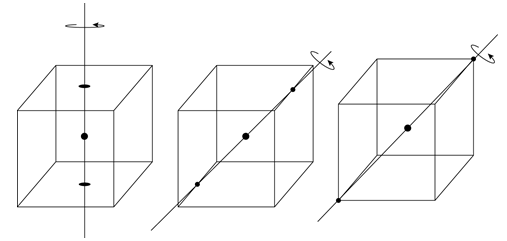
\includegraphics[scale=0.75]{cube-symmetries.jpg}
\end{frame}

\begin{frame}
\frametitle{Application}
	\textbf{Example}. \textit{How many rotational symmetries does a cube have?}
	
	\begin{itemize}
		\item The group of rotations $G$ acts on the set of faces $F$ of the cube.
		\item Every face of the cube is in the orbit of a particular face $f \in F$, so $|O_f|=|F|=6$.
		\item For any face $f \in F$, there are four rotations in $G$ that will preserve $f$, so $|G_f|=4$.
		\item By the Orbit-stabilizer Theorem, $|G|=|G_f| \cdot |O_f| = 4 \cdot 6 = 24$.
		\item Thus, a cube has \textbf{24} rotational symmetries.
	\end{itemize}
\end{frame}
\end{document}